\documentclass{article}
\usepackage{tikz}
\usepackage{amsmath}

\newcommand{\rad}{5}

\begin{document}
\pagenumbering{gobble}
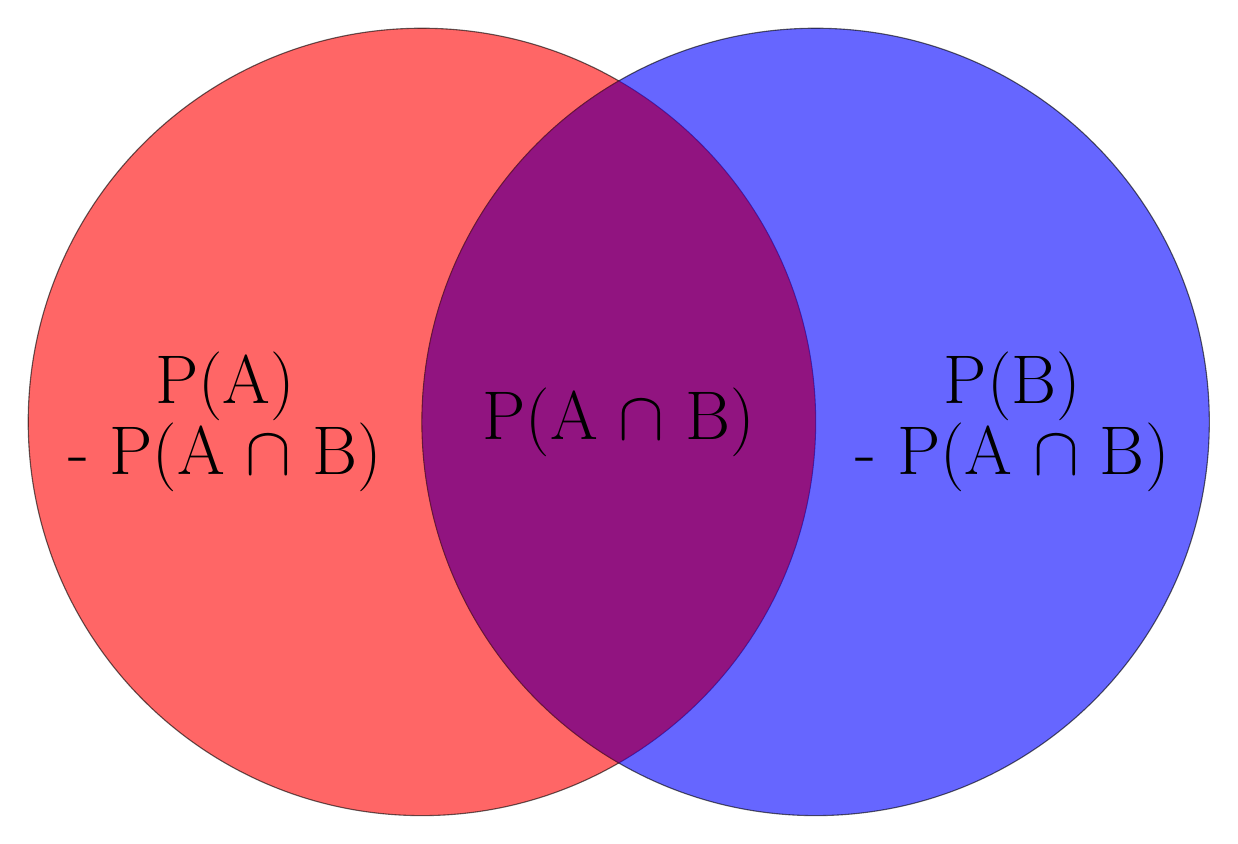
\begin{tikzpicture}
\draw[fill=red, opacity=0.6] (-2.5, 0) circle (5);
\draw[fill=blue, opacity=0.6] (2.5, 0) circle (5);

\begin{scope}
\clip (-2.5, 0) circle (5);
\clip (2.5,  0) circle (5);

\draw[fill=purple, opacity=0.5] (-5, -5) rectangle (5, 5);
\end{scope}

\node[align=center] at (-5, 0) {\Huge P(A) \\\Huge - P(A $\cap$ B)};
\node[align=center] at (5, 0) {\Huge P(B) \\\Huge - P(A $\cap$ B)};
\node[] at (0, 0) {\Huge P(A $\cap$ B)};

\end{tikzpicture}
\end{document}